\documentclass[tikz,border=4pt]{standalone}
% Estilos compartilhados pelos diagramas dos estágios e módulos do Core.
\usetikzlibrary{arrows.meta, positioning, calc, shapes.geometric, fit}

\tikzset{
  >={Stealth[length=2.2mm]},
  bloco/.style={draw, rounded corners=2pt, minimum width=24mm, minimum height=9mm,
                align=center, font=\small, fill=blue!6},
  regpipe/.style={draw, minimum width=9mm, minimum height=48mm, align=center,
                  font=\small, fill=gray!25},
  mux/.style={draw, trapezium, trapezium angle=70, shape border rotate=90,
              minimum height=11mm, minimum width=7mm, inner sep=1pt, align=center,
              font=\scriptsize, fill=orange!15},
  ctrl/.style={draw, rounded corners=2pt, minimum width=24mm, minimum height=9mm,
               align=center, font=\small, fill=green!10},
  opcional/.style={bloco, dashed, fill=yellow!12},
  externo/.style={draw, rounded corners=2pt, minimum width=24mm, minimum height=9mm,
                  align=center, font=\small, fill=red!8},
  dado/.style={->, thick},
  sinal/.style={->, dashed},
  rotulo/.style={font=\scriptsize, midway, above, inner sep=1pt},
  titulo/.style={font=\bfseries\normalsize}
}

\begin{document}
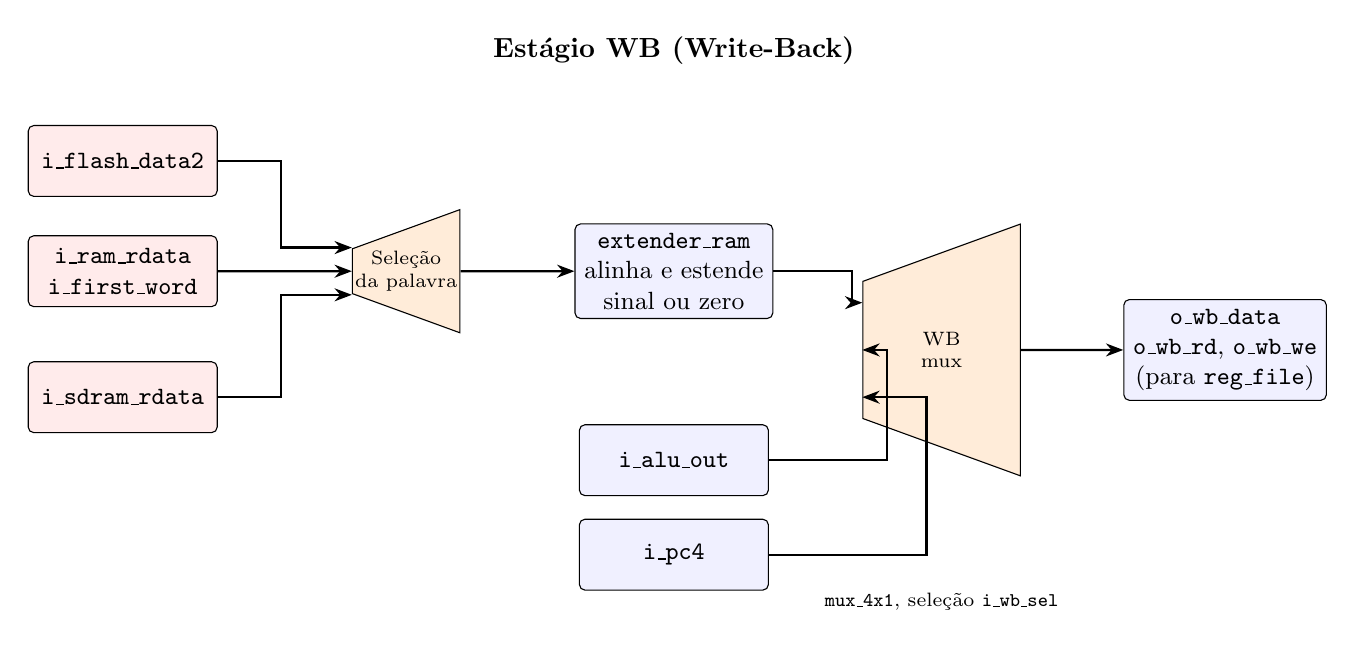
\begin{tikzpicture}
  \node[titulo] at (7,4.6) {Estágio WB (Write-Back)};
  \node[externo] (fl) at (0,3.2) {\texttt{i\_flash\_data2}};
  \node[externo] (ram) at (0,1.8) {\texttt{i\_ram\_rdata}\\\texttt{i\_first\_word}};
  \node[externo] (sd) at (0,0.2) {\texttt{i\_sdram\_rdata}};
  \node[mux] (sel) at (3.6,1.8) {Seleção\\da palavra};
  \node[bloco] (ex) at (7,1.8) {\texttt{extender\_ram}\\alinha e estende\\sinal ou zero};
  \node[bloco] (alu) at (7,-0.6) {\texttt{i\_alu\_out}};
  \node[bloco] (pc4) at (7,-1.8) {\texttt{i\_pc4}};
  \node[mux, minimum height=20mm] (wbm) at (10.4,0.8) {WB\\mux};
  \node[bloco] (out) at (14,0.8) {\texttt{o\_wb\_data}\\\texttt{o\_wb\_rd}, \texttt{o\_wb\_we}\\(para \texttt{reg\_file})};

  \draw[dado] (fl.east) -- ++(0.8,0) |- ([yshift=3mm]sel.west);
  \draw[dado] (ram) -- (sel);
  \draw[dado] (sd.east) -- ++(0.8,0) |- ([yshift=-3mm]sel.west);
  \draw[dado] (sel) -- (ex);
  \draw[dado] (ex.east) -- ++(1.0,0) |- ([yshift=6mm]wbm.west);
  \draw[dado] (alu.east) -- ++(1.5,0) |- ([yshift=0mm]wbm.west);
  \draw[dado] (pc4.east) -- ++(2.0,0) |- ([yshift=-6mm]wbm.west);
  \draw[dado] (wbm) -- (out);
\node[font=\scriptsize] at (10.4,-2.4) {\texttt{mux\_4x1}, seleção \texttt{i\_wb\_sel}};
\end{tikzpicture}
\end{document}
